\chapter{Обзор литературы}


\section{Методика поиска литературы}

Поиск литературы по тематике мониторинга лазерной сварки проводился преимущественно с использованием систем: \textit{Google Scholar}, \textit{Scopus} и \textit{Web of Science}. Дополнительно отбор релевантных публикаций выполнялся по спискам литературы в уже найденных статьях, прежде всего в обзорных работах, что позволило выявить как более ранние фундаментальные исследования, так и современные публикации, непосредственно связанные с анализом оптических сигналов при сварке.

Основное внимание уделялось работам, связанным с регистрацией и интерпретацией оптических сигналов в процессе лазерной сварки. В качестве базовых поисковых запросов использовались сочетания, ориентированные на мониторинг излучения, спектральный анализ и диагностику процесса, в частности: \textit{laser welding optical emission monitoring}, \textit{in process monitoring laser welding spectroscopy}, \textit{optical monitoring of laser welding process}, \textit{plasma emission monitoring laser welding}. Наряду с обзорными статьями рассматривались и экспериментальные работы, в которых исследовались конкретные методы регистрации сигналов, способы извлечения признаков и алгоритмы распознавания дефектов.

Критерием включения публикаций в обзор литературы являлось наличие оптических датчиков, используемых для наблюдения за процессом сварки, и связь работы с задачами оценки качества шва, глубины проплавления, устойчивости процесса или выявления дефектов. При отборе материалов особый акцент делался на исследованиях, в которых оптические данные не только регистрировались, но и подвергались дальнейшей обработке методами анализа сигналов, статистического извлечения признаков и машинного обучения. Такой подход обусловлен тем, что именно сочетание средств оптической регистрации и современных алгоритмов обработки данных соответствует задачам настоящей работы.


\section{Типы оптических датчиков, применяемых для мониторинга лазерной сварки}

Оптический мониторинг лазерной сварки основан на регистрации сигналов, непосредственно связанных с физическими процессами в зоне взаимодействия лазерного излучения с материалом. К числу таких процессов относятся: тепловое излучение расплава, излучение плазменного факела, отражённое лазерное излучение, а также изменение геометрии ванны расплава и парогазового канала. В литературе наибольшее распространение получили: фотодиодные, спектрометрические, камерные и пирометрические системы наблюдения~\cite{wu2022progress,huang2025laser}.

\subsection{Фотодиодные датчики}

Фотодиоды являются одним из наиболее распространённых средств регистрации оптических сигналов при лазерной сварке. Их широкое применение обусловлено простой конструкцией, высокой скоростью отклика, низкой стоимостью и удобством интеграции в промышленное оборудование~\cite{wu2022progress,huang2025laser}. В отличие от спектрометров, фотодиоды регистрируют не полный спектр излучения, а интегральную интенсивность в заданном спектральном диапазоне, который определяется собственной спектральной чувствительностью датчика или установленными оптическими фильтрами. На рис.~\ref{fig:photodiode_sensitivity} приведен пример областей чувствительности фотодиодов.

\begin{figure}[H]
    \centering
    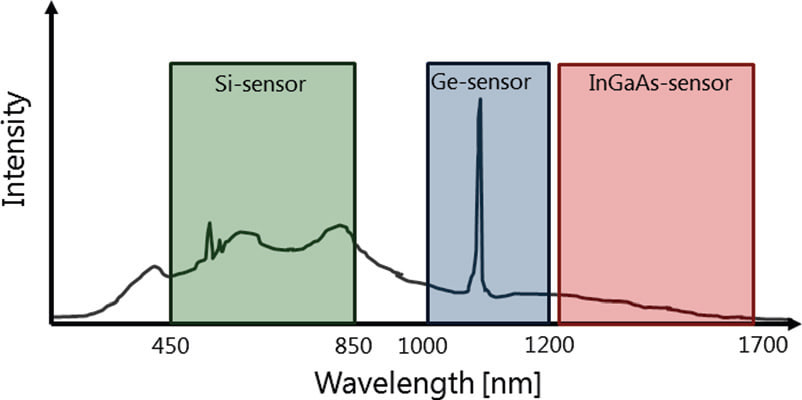
\includegraphics[width=0.75\linewidth]{figures/Чувствительность фотодиодов.jpg}
    \caption{Сравнение чувствительности светодиодов и спектра излучения области сварки~\cite{vakili2017wavelet}.}
    \label{fig:photodiode_sensitivity}
\end{figure}

В зависимости от выбранного диапазона фотодиодные системы могут регистрировать различные компоненты сигнала. Сигналы в ультрафиолетовой и видимой области обычно связаны с излучением плазменного факела и испарённого материала, тогда как ближний инфракрасный диапазон и отражённое лазерное излучение в большей степени чувствительны к энергетическому взаимодействию лазера с поверхностью, состоянию расплава и динамике парогазового канала~\cite{wu2022progress,huang2025laser}. В ряде работ фотодиоды использовались как в одноканальной конфигурации, так и в виде набора датчиков, каждый из которых регистрирует отдельный спектральный диапазон.

Характерным примером ранней многоканальной фотодиодной системы является работа~\cite{park2001fuzzy}, где использовались два ультрафиолетовых и один инфракрасный канал. Такая конфигурация позволяла регистрировать излучение плазмы, а также оценивать изменение поглощаемой плотности мощности и положения фокуса. Важным достоинством фотодиодного подхода является возможность перехода от сложной спектрометрии к более простой системе, сохраняющей чувствительность к наиболее информативным диапазонам.

В работе~\cite{kawahito2004process} фотодиоды использовались для регистрации отражённого сигнала и теплового излучения, причём показано, что эти сигналы непосредственно связаны с формированием парогазового канала и размером зоны проплавления. Практическая ценность фотодиодных систем в связана не только с простотой их аппаратной реализации, но и с возможностью получать сигнал с малой задержкой. Для задач оперативного мониторинга это особенно важно, поскольку признак дефекта должен быть доступен непосредственно во время сварки, а не только после завершения прохода. Близкий подход использован в работе~\cite{olsson2011advances}, где отражённое излучение рассматривалось не как самостоятельная физическая величина, а как источник статистических признаков: анализировались дисперсия сигнала и изменение формы импульсов, связанные со стабильностью процесса.

Отдельный интерес представляют работы, в которых фотодиодный сигнал анализировался как динамический процесс. В~\cite{mrvna2013correlation} фотодиод применялся для изучения связи между глубиной парогазового канала и частотными характеристиками оптического излучения. Даже при отсутствии спектрального разрешения фотодиодный канал может сохранять информацию о колебаниях ванны расплава и парогазового канала. Однако эта информация проявляется не столько в среднем уровне сигнала, сколько в его временной и временно-частотной структуре, что обосновывает применение частотного и вейвлет-анализа~\cite{vakili2017wavelet,fang2004wavelet}.

Таким образом, фотодиодный подход нельзя сводить только к более дешёвой замене спектрометра. В работе~\cite{zhang2019low} низкозатратная система на основе двух фотодиодов, регистрирующих видимое излучение и отражённый лазерный сигнал, использовалась для различения нескольких состояний сварки, включая качественный шов и характерные дефекты. Для промышленного мониторинга это принципиально: фотодиоды образуют отдельный класс высокоскоростных оптических датчиков, пригодных для построения систем контроля, если интегральные сигналы сопровождаются содержательной цифровой обработкой.

\begin{figure}[H]
    \centering
    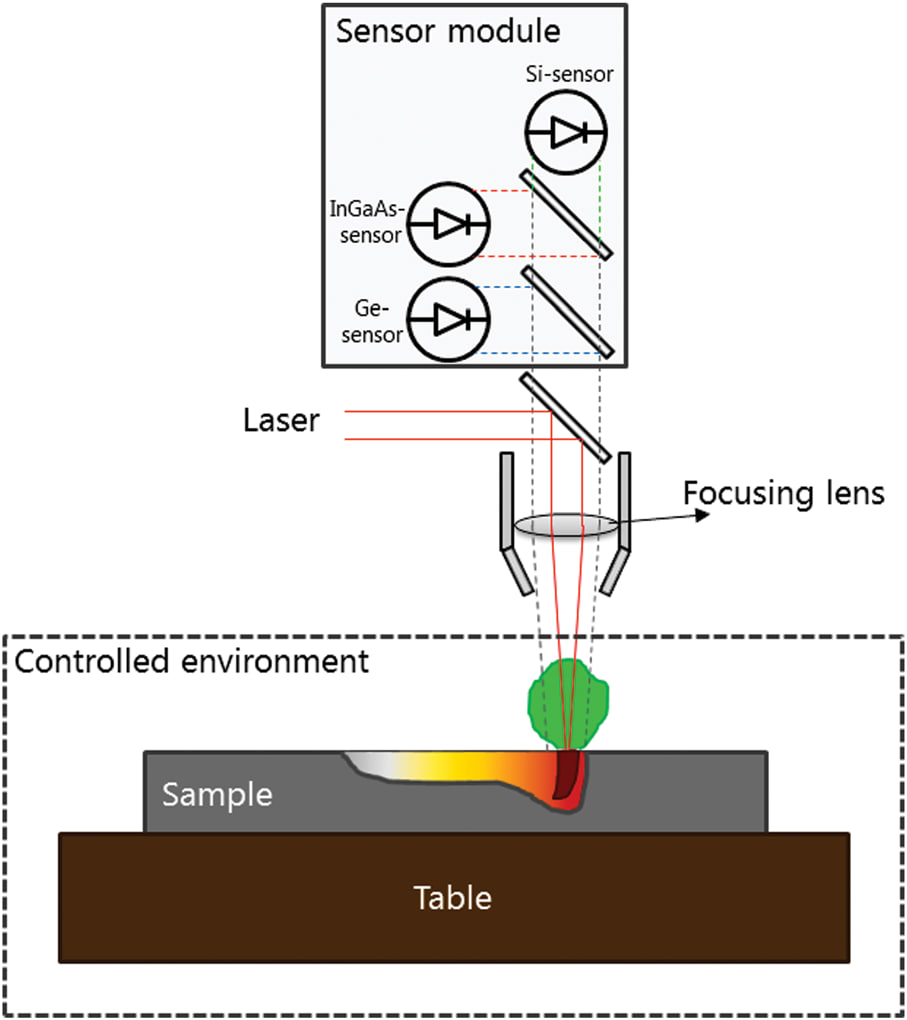
\includegraphics[width=0.75\linewidth]{figures/Фотодиоды.jpg}
    \caption{Пример схемы фотодиодной системы мониторинга лазерной сварки с коаксиальным наблюдением~\cite{you2014review}.}
    \label{fig:photodiode_setup}
\end{figure}



\subsection{Спектрометрические системы}

В отличие от фотодиодов, спектрометр сохраняет распределение интенсивности излучения по длинам волн. Поэтому исследователь получает доступ не только к интегральному уровню сигнала, но и к форме спектра, отдельным спектральным линиям, их относительным интенсивностям и производным физическим параметрам, например электронной температуре плазмы~\cite{wu2022progress,huang2025laser,sebestova2012non}. Именно это делает спектрометрический канал наиболее информативным с точки зрения физической интерпретации, но одновременно усложняет как аппаратную часть, так и последующую обработку данных.

Одним из первых направлений применения спектрометров при мониторинге лазерной сварки стала оптическая эмиссионная спектроскопия плазмы. В работе~\cite{bruncko2003monitoring} анализировались интенсивности отдельных спектральных линий и их отношения; эти параметры использовались для различения режимов сварки и сопоставления спектрального отклика с качеством шва. Сходная логика реализована в~\cite{sebestova2012non}, где по отношению спектральных линий рассчитывалась температура плазмы, после чего исследовалась её связь с глубиной проплавления и появлением дефектов.

Наиболее показательной для задачи физически интерпретируемого мониторинга является работа~\cite{konuk2011closed}. В ней спектральный сигнал был преобразован в количественный параметр --- электронную температуру плазмы, которая затем использовалась в замкнутом контуре управления глубиной проплавления. Этот пример важен тем, что демонстрирует полную диагностическую цепочку: регистрация оптического сигнала, вычисление физически осмысленного признака, оценка состояния процесса и последующее изменение режима.

Преимущество спектрометрического подхода особенно заметно при выборе информативных спектральных диапазонов и при анализе природы регистрируемого излучения. Вместе с тем высокая информативность достигается за счёт более сложной измерительной схемы, меньшей частоты регистрации по сравнению с фотодиодами и увеличения размерности данных~\cite{wu2022progress, huang2025laser}. Поэтому в современных работах спектрометрический сигнал всё чаще рассматривается не только как источник отдельных физических параметров, но и как высокоразмерное признаковое описание, требующее автоматического
извлечения информативных характеристик.

Такой подход реализован, например, в работе~\cite{8756200}, где полный спектральный сигнал использовался для автоматического распознавания дефектов с помощью глубокой модели на основе SAE. Существенно, что здесь спектрометр рассматривается уже не только как средство физического анализа отдельных линий, но и как источник высокоразмерной информации, пригодной для построения диагностических моделей на основе экспериментальных данных. В этом смысле спектрометрические системы занимают промежуточное положение между классической физической интерпретацией и современными методами интеллектуальной обработки.

\begin{figure}[H]
    \centering
    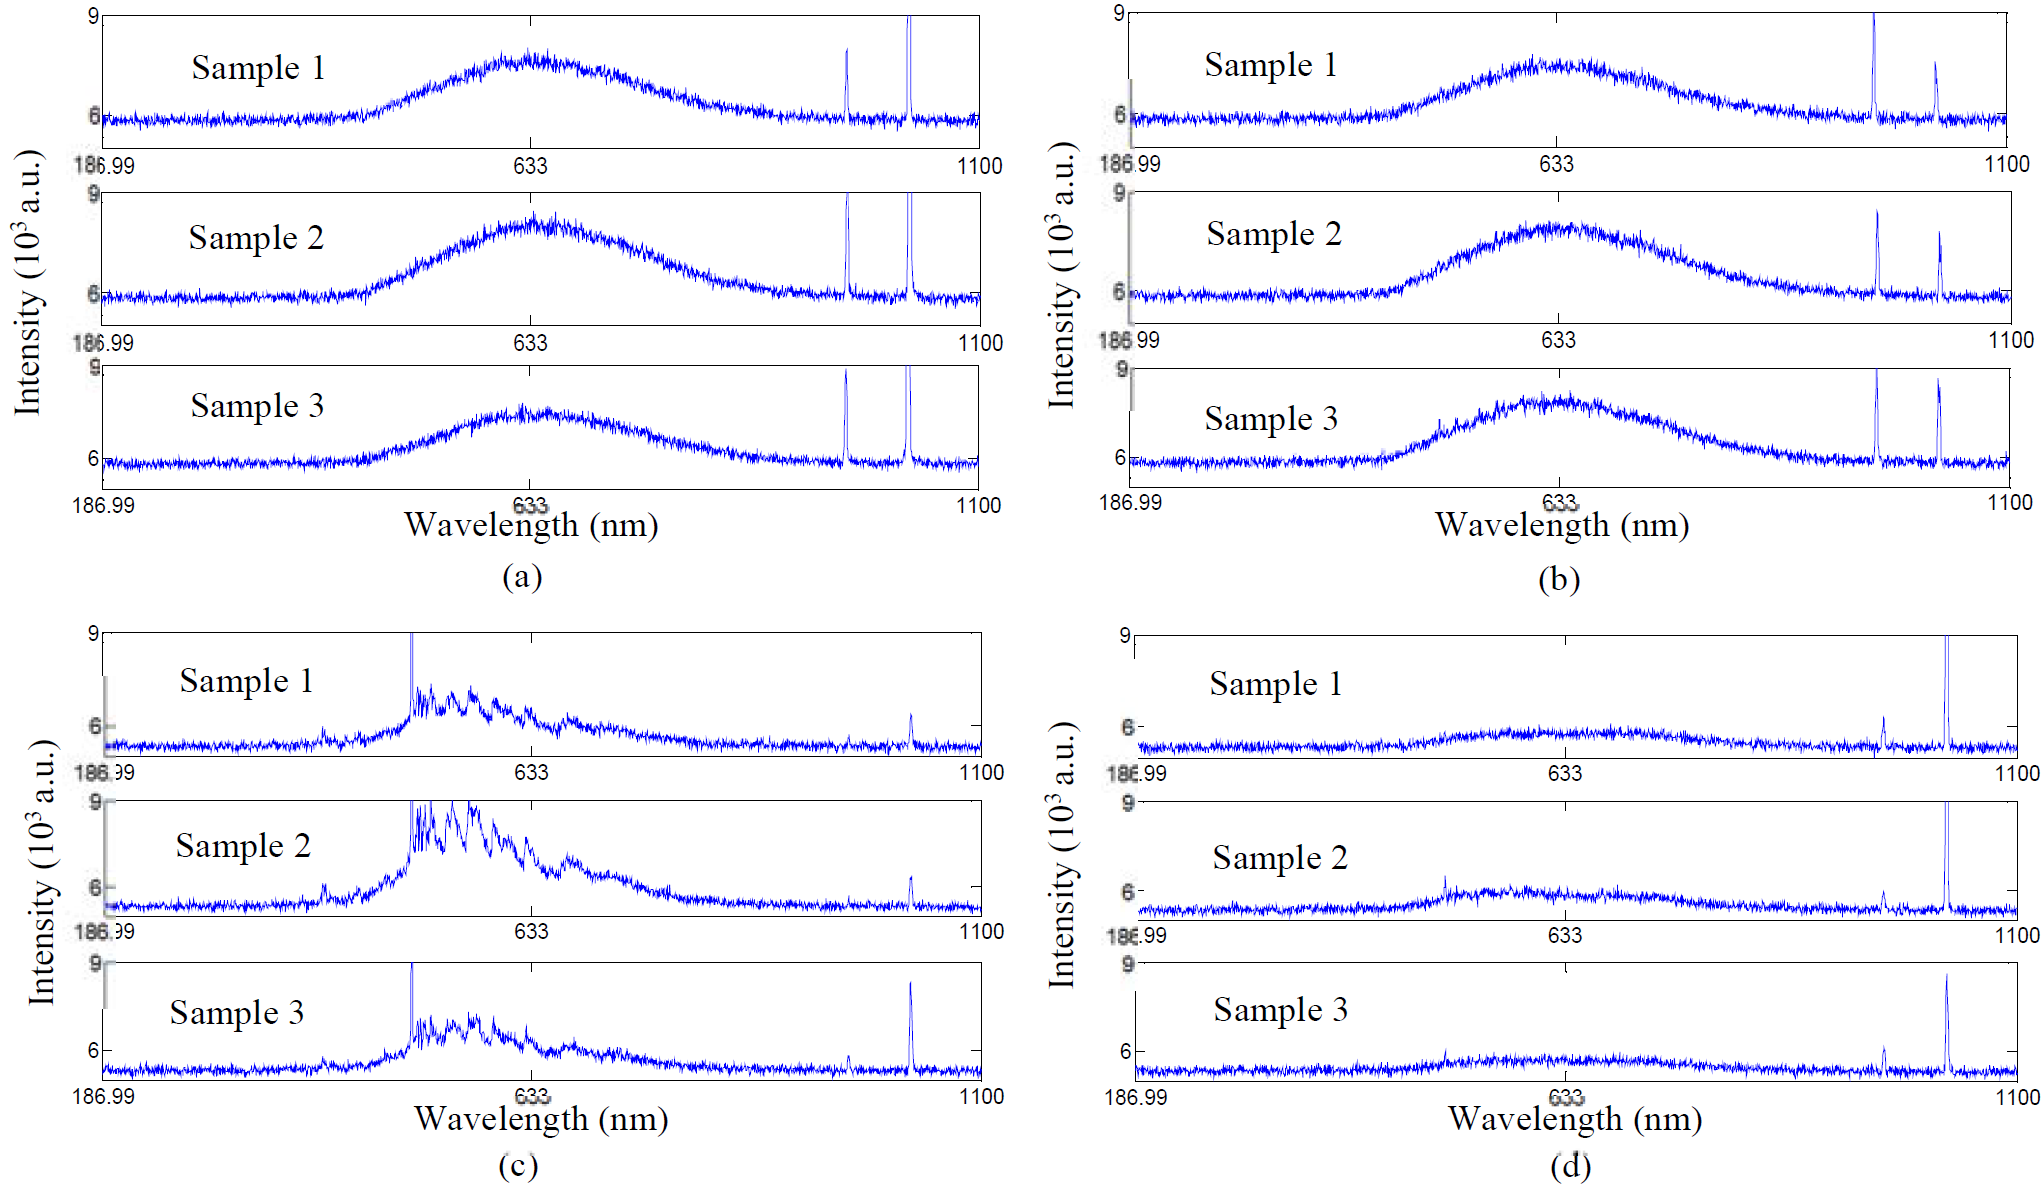
\includegraphics[width=1\textwidth]{figures/Примеры спектров.png}
    \caption{Примеры спектров для различных дефектов лазерной сварки (a)~Качественный сварной шов; (b)~Прожог; (c)~Превышение выпуклости; (d)~Подрез~\cite{8756200}.}
    \label{fig:spectra_welding_defects}
\end{figure}

\subsection{Камерные системы}

Камерные системы отличаются от фотодиодов и спектрометров тем, что дают пространственно распределённую информацию о процессе. Если фотодиоды и спектрометры регистрируют преимущественно амплитудные и спектральные характеристики излучения, то камеры позволяют непосредственно наблюдать геометрию ванны расплава, форму плазменного факела, брызги и размеры входа в парогазовый канал~\cite{wu2022progress,huang2025laser}. Это делает их особенно ценными в тех случаях, когда требуется анализ морфологии процесса.

В задачах визуального мониторинга применяются ПЗС-камеры, КМОП-камеры и высокоскоростные камеры, а также схемы с внешней подсветкой, позволяющие наблюдать область парогазового канала и ванну расплава на фоне интенсивного собственного излучения процесса. В работе~\cite{wang2020monitoring} в качестве диагностических параметров рассматривались площадь входа в парогазовый канал и ширина ванны расплава. В этом случае оценка состояния сварки опирается не на интегральную интенсивность излучения, а на геометрическое описание зоны взаимодействия лазерного пучка с материалом.

Более сложная схема наблюдения рассмотрена в работе~\cite{ZHANG2019671}, где камеры ультрафиолетового и видимого диапазонов использовалась совместно с системой вспомогательной подсветки. Такая конфигурация позволяла раздельно выделять признаки плазменного факела, брызг и парогазового канала. В мультисенсорных системах подобный подход дополняет фотодиодные и спектральные измерения пространственной информацией о процессе.

\begin{figure}[H]
    \centering
    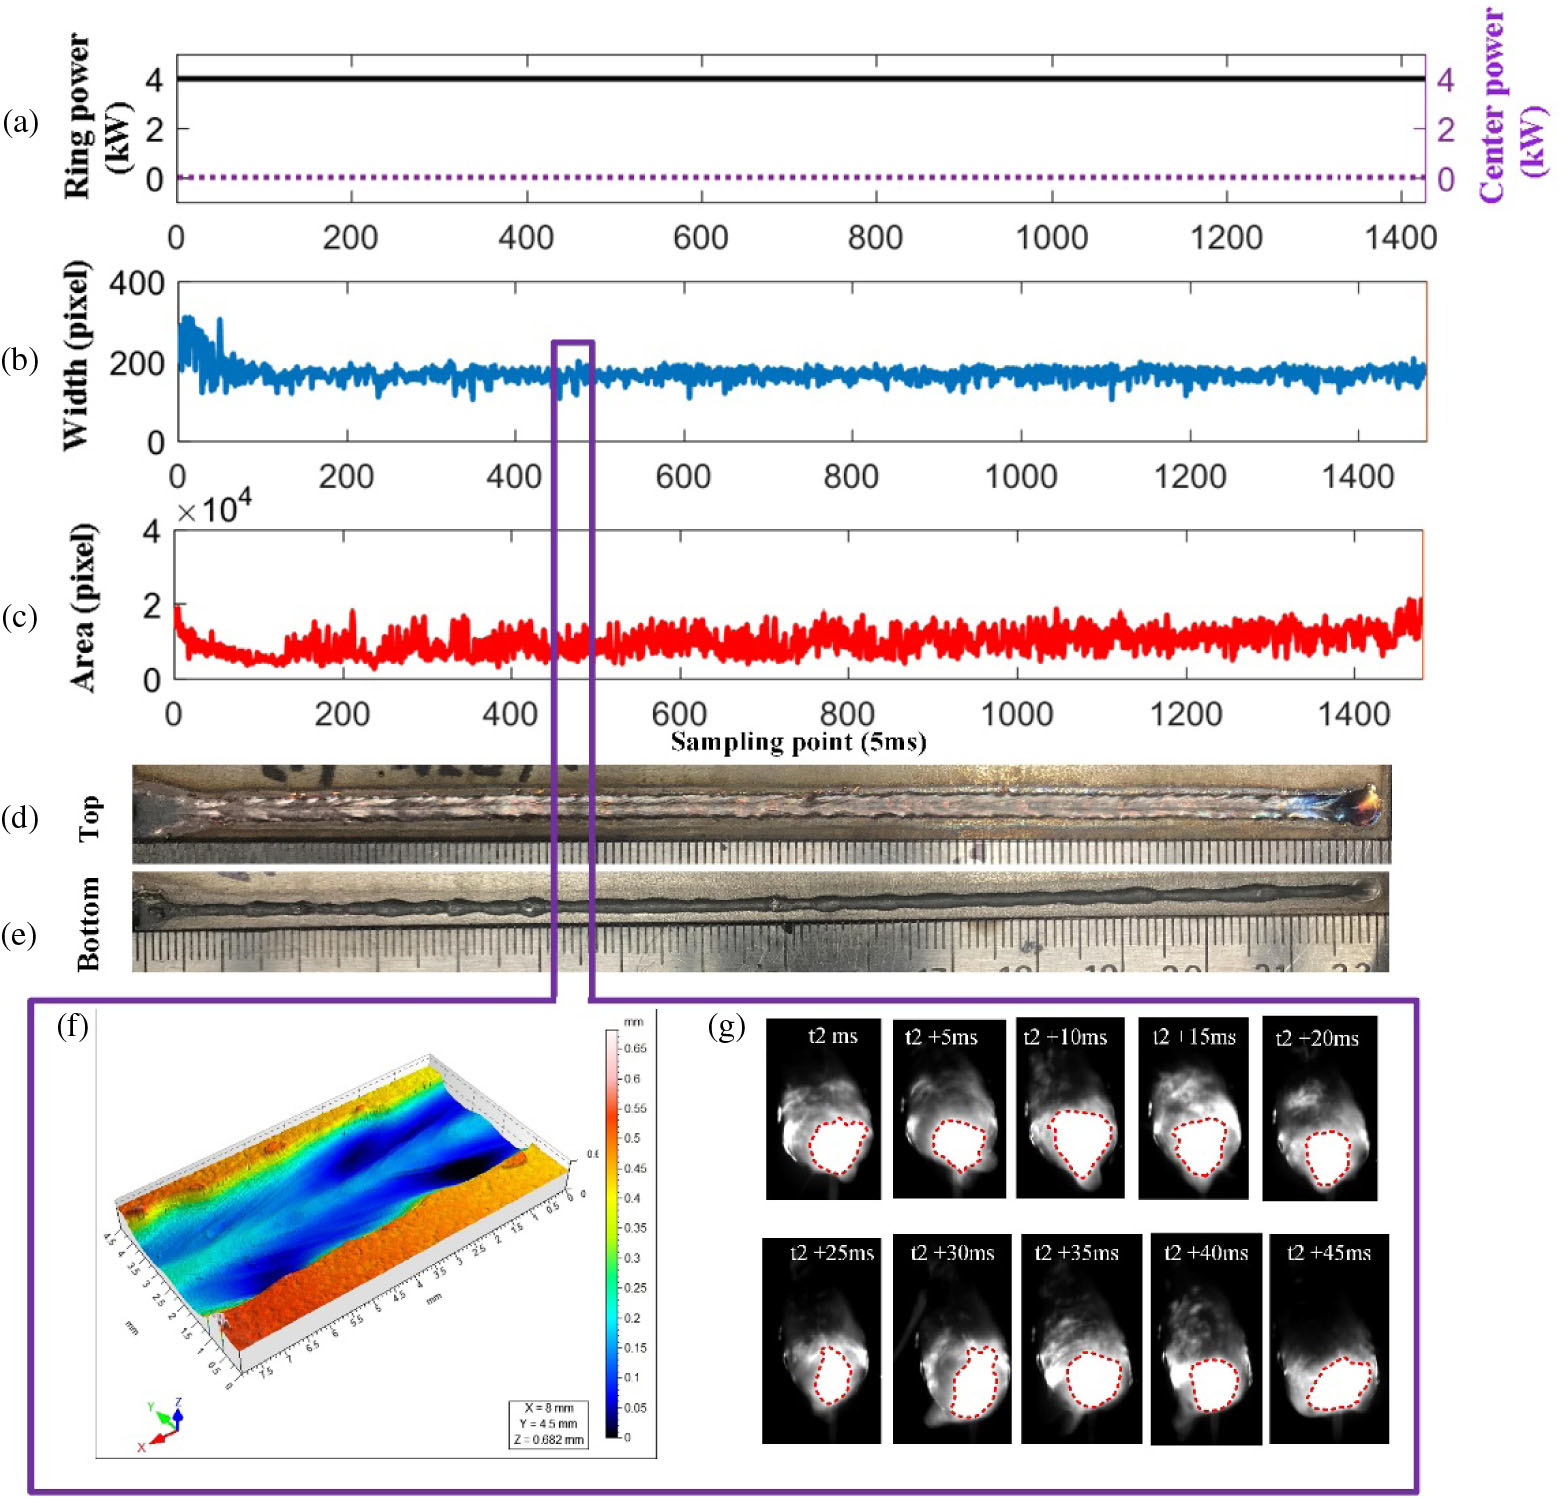
\includegraphics[width=1\textwidth]{figures/Камера.png}
    \caption{Использование камеры для наблюдения за ванной расплава и парогазовым каналом.
    (a)~изменение мощности;~(b) ширина ванны расплава; (c)~площадь входного отверстия в парогазовый канал; (d)~верхняя поверхность сварного шва; (e)~нижняя поверхность сварного шва; (f)~трёхмерный профиль сварного шва при сварке кольцевым лучом; (g)~изображения ванны расплава при сварке кольцевым лучом~\cite{wang2020monitoring}.}
    \label{fig:camera_monitoring}
\end{figure}

Главным достоинством камерных систем является наглядность и высокая информативность в отношении геометрии процесса. Однако это достоинство сопровождается рядом ограничений: повышенными требованиями к освещению, высокой чувствительностью к засветке и плазменным выбросам, а также необходимостью достаточно сложной обработки изображений~\cite{wu2022progress,huang2025laser}. Поэтому камеры часто рассматриваются не как единственный сенсор, а как один из элементов многоканальной системы мониторинга.

\subsection{Пирометры и инфракрасные системы наблюдения}

Пирометры и инфракрасные системы занимают особое место среди оптических датчиков, поскольку ориентированы прежде всего на регистрацию теплового излучения и оценку температурного состояния зоны сварки~\cite{wu2022progress,huang2025laser}. По сравнению с камерами и спектрометрами они обычно предоставляют менее детальную информацию о структуре процесса, однако могут быть весьма полезны для оценки температуры расплава, ширины шва и распределения тепла.

Сильной стороной пирометрических систем является бесконтактность, относительная простота и ориентация на один из фундаментальных параметров процесса --- температуру. В то же время их применение осложняется зависимостью результатов от коэффициента излучения материала, влиянием плазмы и ограниченной возможностью прямого выявления локальных дефектов~\cite{wu2022progress}. По этой причине в задачах комплексного мониторинга пирометры и инфракрасные системы чаще используются как вспомогательные средства, дополняющие фотодиодные, спектрометрические и визуальные наблюдения.

\subsection{Расположение датчиков}

Не менее важным фактором, чем тип датчика, является его расположение относительно зоны сварки. В литературе наиболее часто встречаются коаксиальные, боковые и комбинированные схемы наблюдения~\cite{wu2022progress,huang2025laser}. Коаксиальная схема удобна тем, что позволяет регистрировать сигнал непосредственно вдоль оси лазерного воздействия и хорошо интегрируется в промышленную оптику. Именно поэтому фотодиоды для регистрации отражённого сигнала и видимого излучения часто располагаются через светоделитель внутри сварочной головы~\cite{zhang2019low}.

Боковое или наклонное расположение датчиков чаще применяется в спектрометрических и визуальных системах. Оно позволяет лучше наблюдать плазменный факел, боковую геометрию ванны расплава и излучение из зоны парогазового канала, однако увеличивает зависимость измерений от геометрии установки и условий экранирования~\cite{konuk2011closed,wang2020monitoring}. В частности, для спектрометрии положение коллиматора и угол наблюдения могут существенно влиять на интерпретацию сигнала.

Комбинированные схемы стремятся объединить преимущества нескольких типов датчиков. В работе~\cite{you2014multisensor} использована многосенсорная архитектура, включающая фотодиоды, камеры и спектрометр. Подобный подход позволяет одновременно учитывать быстрые интегральные сигналы, геометрические признаки и спектральную информацию. Аналогичная идея развивается и в~\cite{ZHANG2019671}, где несколько оптических каналов используются для получения более полного описания состояния процесса. Несмотря на очевидные преимущества, такие системы оказываются более сложными как с точки зрения аппаратной реализации, так и с точки зрения последующей обработки данных.

\begin{figure}[H]
    \centering
    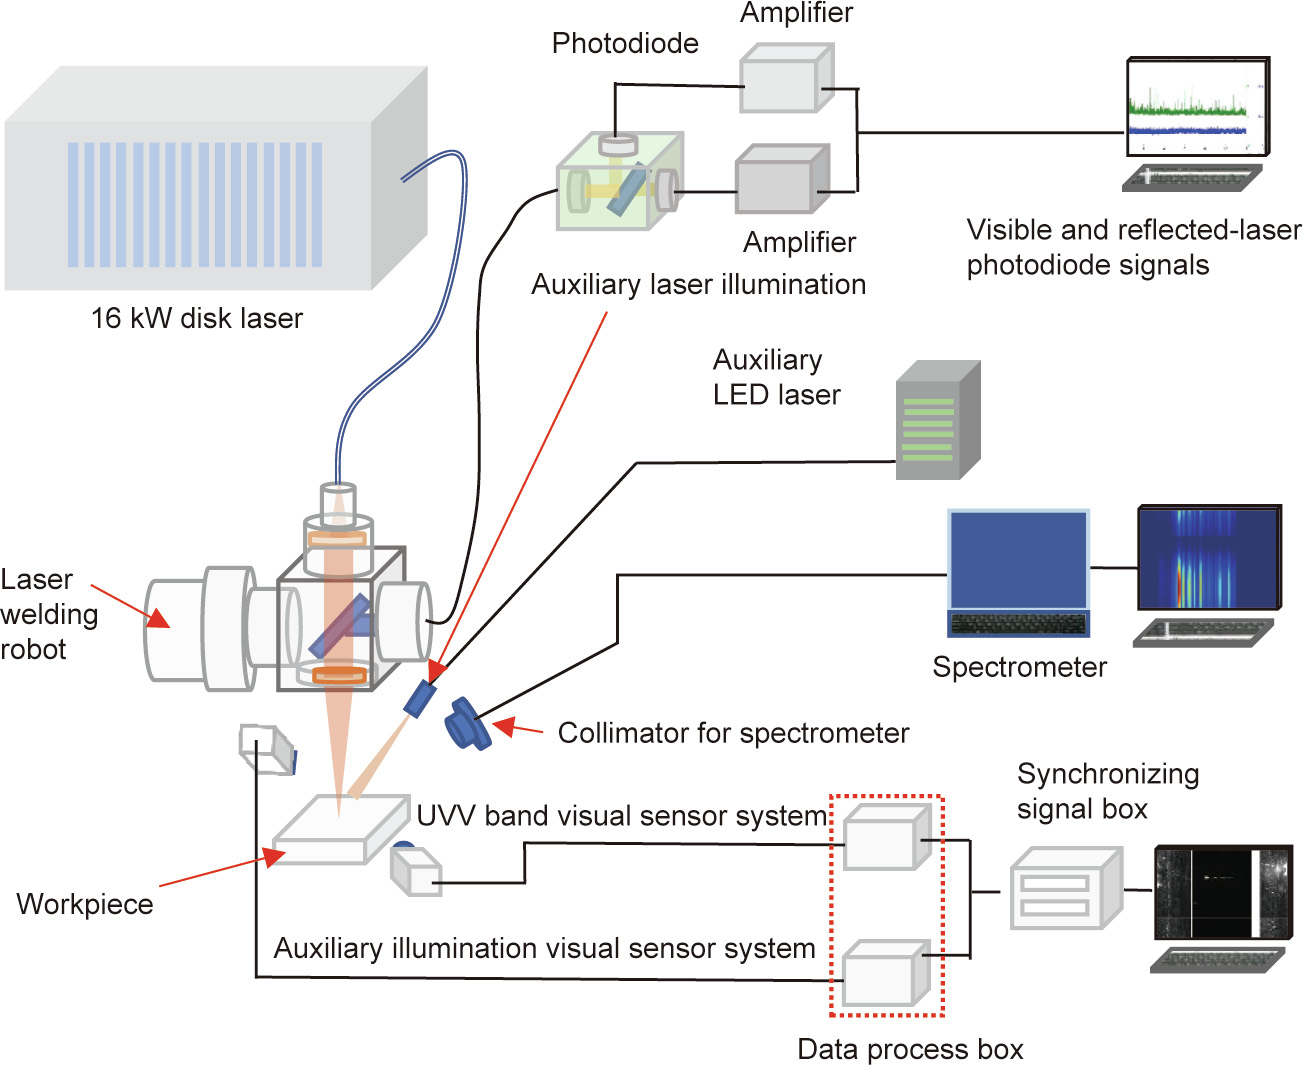
\includegraphics[width=0.75\textwidth]{figures/Мультисенсор.png}
    \caption{Пример экспериментальной установки с мультисенсорной системой~\cite{ZHANG2019671}.}
    \label{fig:multisensor}
\end{figure}

\subsection{Итоги рассмотрения методов мониторинга}

Таким образом, различные типы оптических датчиков регистрируют разные аспекты процесса лазерной сварки. Фотодиоды обеспечивают высокую скорость и простоту реализации, спектрометры дают наиболее богатую спектральную информацию, камеры позволяют непосредственно наблюдать геометрию ванны расплава и парогазового канала, а пирометры ориентированы на температурные характеристики процесса~\cite{wu2022progress,huang2025laser}. Выбор конкретного типа датчика определяется компромиссом между информативностью, скоростью, стоимостью и сложностью обработки данных. В большинстве современных исследований наблюдается тенденция к объединению нескольких каналов регистрации, однако для практических задач по-прежнему сохраняется интерес к более простым и быстрым системам, прежде всего фотодиодным.




\section{Методы анализа оптических данных при мониторинге лазерной сварки}

После регистрации оптических сигналов возникает задача их интерпретации. Зависимость напряжения на фотодиоде от времени, спектр излучения плазменного факела или последовательность изображений зоны сварки сами по себе ещё не дают прямого ответа на вопрос о качестве шва. Необходим этап обработки, на котором исходные данные преобразуются в параметры, связанные с глубиной проплавления, устойчивостью процесса, формированием области парогазового канала и вероятностью появления дефектов. В современной литературе методы анализа оптических данных обычно развиваются по трём основным направлениям: прямая физическая корреляция, извлечение признаков и машинное обучение~\cite{wu2022progress,huang2025laser,you2014review}.

Такая классификация удобна не только с методической точки зрения, но и с практической. На первом уровне логично связать сигнал с процессом максимально прозрачно, опираясь на физическую интерпретацию измеряемой величины. На втором уровне акцент переносится на формирование компактного и устойчивого описания сигнала в виде набора признаков. На третьем уровне полученное представление используется для автоматической классификации состояний процесса и дефектов. Переход от физически интерпретируемых признаков к моделям, построенным на основе экспериментальных данных, во многом определяет современное развитие систем мониторинга лазерной сварки~\cite{wu2022progress,huang2025laser}.

\subsection{Прямая физическая корреляция}

Наиболее очевидный путь анализа состоит в поиске параметра сигнала, который можно непосредственно связать с физическим состоянием зоны сварки. Такой подход особенно характерен для ранних работ по спектрометрии и фотодиодному мониторингу, где исследователи стремились не столько классифицировать дефекты, сколько понять, каким образом изменение сигнала связано с изменением режима сварки.

Для спектрометрических систем характерен анализ отдельных спектральных линий и их отношений. В работах~\cite{bruncko2003monitoring,sebestova2012non,konuk2011closed,connolly2000optical} показано, что интенсивности линий излучения плазмы и их соотношения изменяются при переходе между режимами сварки и могут быть связаны с глубиной проплавления. В работе~\cite{konuk2011closed} эта связь была использована уже не только для диагностики: спектральные данные преобразовывались в электронную температуру плазмы, после чего данный параметр применялся для регулирования мощности лазера. Тем самым спектральный сигнал рассматривался как измеряемая величина, пригодная для построения обратной связи.

Аналогичная идея встречается и в фотодиодных системах. В работах~\cite{kawahito2004process,kawahito2009process} отражённое и тепловое излучение регистрировались отдельными каналами и использовались как индикаторы формирования расплава и области парогазового канала. В таком случае диагностическая информация извлекается не из полного спектра, а из изменения интегрального оптического отклика во времени.

Существенный интерес представляет и частотная интерпретация сигнала. В статье~\cite{geiger2008high} показано, что после преобразования Фурье по времени в фотодиодном сигнале выделяются характерные частоты, связанные с колебаниями расплава и области парогазового канала. В работе~\cite{mrvna2013correlation} эта идея была развита за счёт применения кратковременного преобразование Фурье: форма спектра и агрегированный параметр, построенный по его распределению, использовались для оценки глубины парогазового канала. Важность подобных работ состоит в том, что они вводят в анализ сигнала не только уровень интенсивности, но и динамическую структуру процесса.


Таким образом, подход прямой физической корреляции остаётся чрезвычайно ценным благодаря своей интерпретируемости. Однако его возможности ограничены. Один параметр сигнала, как правило, не позволяет надёжно различать несколько дефектных состояний, а сама зависимость часто требует повторной настройки при изменении материала, толщины или конфигурации датчика~\cite{wu2022progress,huang2025laser}. Поэтому дальнейшее развитие методов мониторинга закономерно связано с переходом к многомерному описанию сигнала.

\subsection{Извлечение признаков}

Предполагается, что исходный сигнал содержит большое количество избыточной или слабоинформативной информации, тогда как для диагностики следует выделить компактный набор характеристик, наиболее чувствительных к изменению режима сварки.

В общем случае результат извлечения признаков можно представить в виде вектора
\[
\mathbf{z} = [z_1, z_2, \dots, z_n],
\]
где \(z_i\) являются статистическими, спектральными, временно-частотными или геометрическими характеристиками сигнала. Качество последующего анализа во многом определяется тем, насколько удачно выбрано это пространство признаков.

\subsubsection{Признаки во временной области}

Наиболее простыми являются признаки во временной области. К ним относятся среднее значение, максимум, дисперсия, среднеквадратичное отклонение, асимметрия, эксцесс, длительность отдельных событий и другие статистические характеристики. Их преимущество состоит в низкой вычислительной сложности и удобстве применения в системах реального времени.

Подход такого типа использовался уже в ранних работах. В статье~\cite{park2001fuzzy} фотодиодные сигналы в ультрафиолетовом и инфракрасном диапазонах сравнивались с эталонными зависимостями, а отклонения использовались как входы для нечеткой системы распознавания. В работе~\cite{olsson2011advances} статистические параметры отражённого сигнала, в частности дисперсия и форма импульса, рассматривались как признаки стабильности процесса. Эти исследования показали, что даже простые статистические характеристики могут быть чувствительны к дефектному формированию шва.

Более систематический подход представлен в статье~\cite{LEE2020307}, где для спектрального сигнала рассчитывались среднее, среднеквадратичное отклонение, пик, асимметрия и эксцесс, а затем выполнялось ранжирование признаков по критерию Фишера. Эта работа важна тем, что показывает: даже на уровне базовых статистик полезно не просто вычислить как можно больше параметров, а отобрать из них наиболее информативные.

Тем не менее временные признаки имеют и очевидные ограничения. Они хорошо отражают уровень сигнала и его изменчивость, но слабо описывают внутреннюю структуру нестационарного процесса. Для лазерной сварки, где существенную роль играют колебания ванны расплава, плазмы и области парогазового канала, этого часто недостаточно.

\subsubsection{Частотные и временно-частотные признаки}

Следующий уровень анализа связан с переходом в частотную или временно-частотную область. Для лазерной сварки это особенно важно, поскольку нестабильности процесса часто проявляются не только изменением амплитуды сигнала, но и перестройкой его спектрального состава.

Частотный анализ позволяет выделить диапазоны, связанные с колебаниями ванны расплава и области парогазового канала~\cite{geiger2008high,mrvna2013correlation}. Однако сигналы лазерной сварки являются нестационарными, поэтому наибольший интерес вызывают методы, учитывающие одновременно и время, и частоту. К ним относятся кратковременное преобразование Фурье, дискретное вейвлет-преобразование и вейвлет-пакетное разложение.


\begin{figure}[H]
    \centering

    \begin{minipage}[t]{0.32\textwidth}
        \centering
        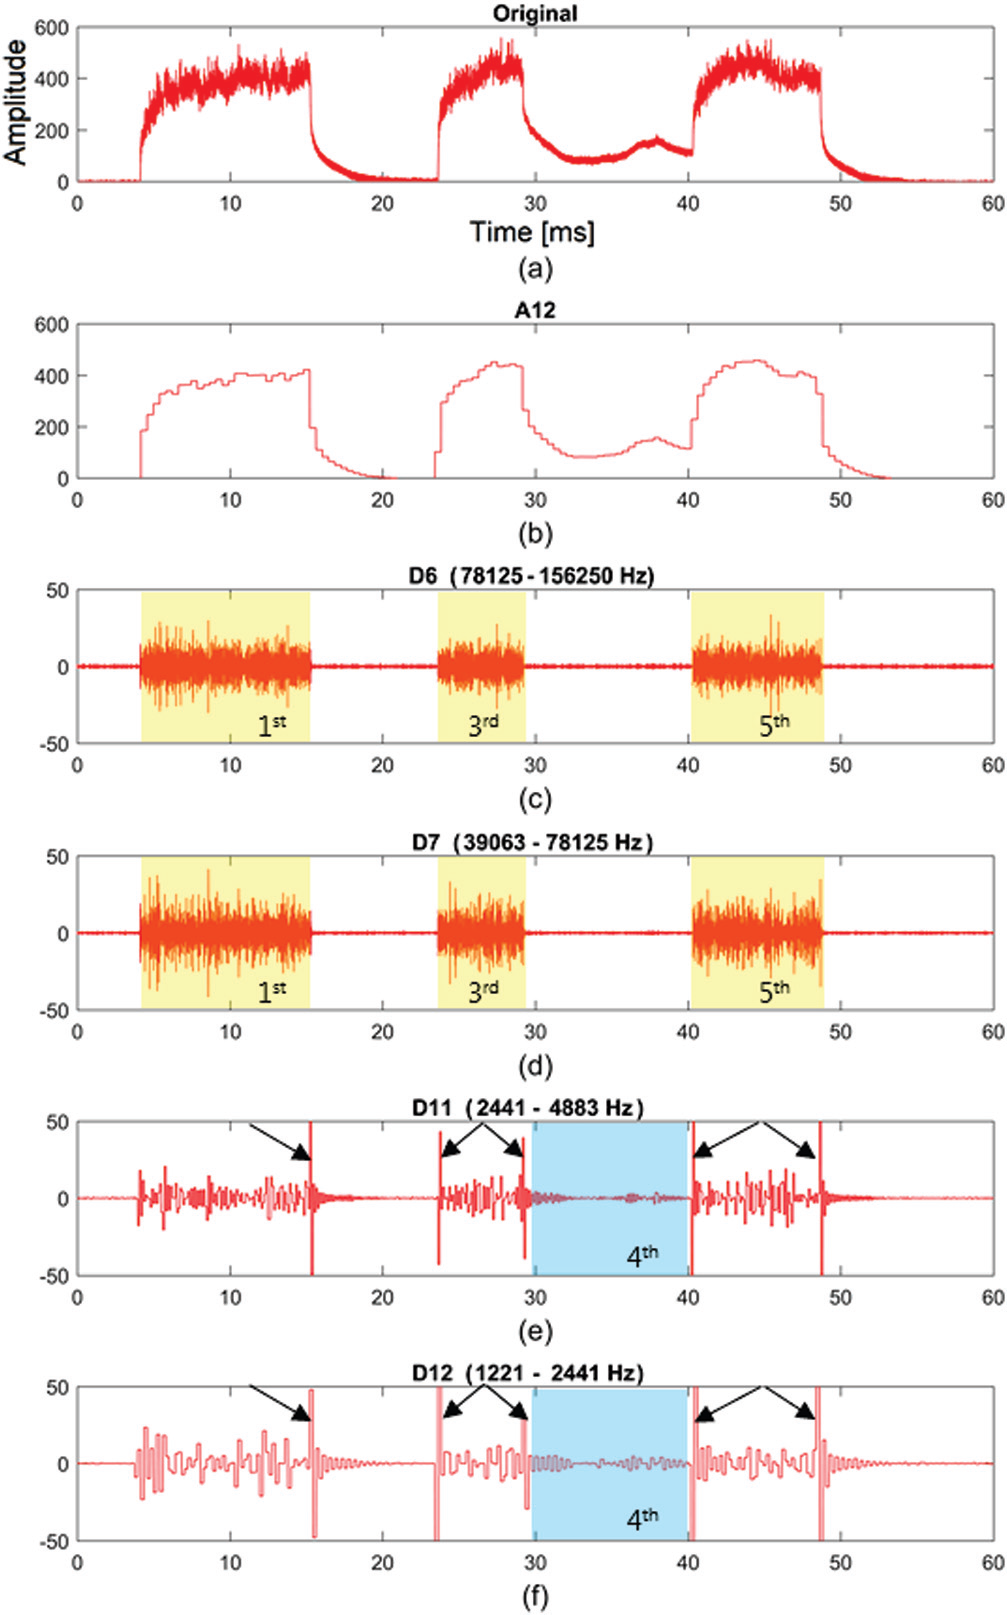
\includegraphics[width=\textwidth]{figures/Wavelet1.png}
        \subcaption{InGaAs}
    \end{minipage}
    \hfill
    \begin{minipage}[t]{0.32\textwidth}
        \centering
        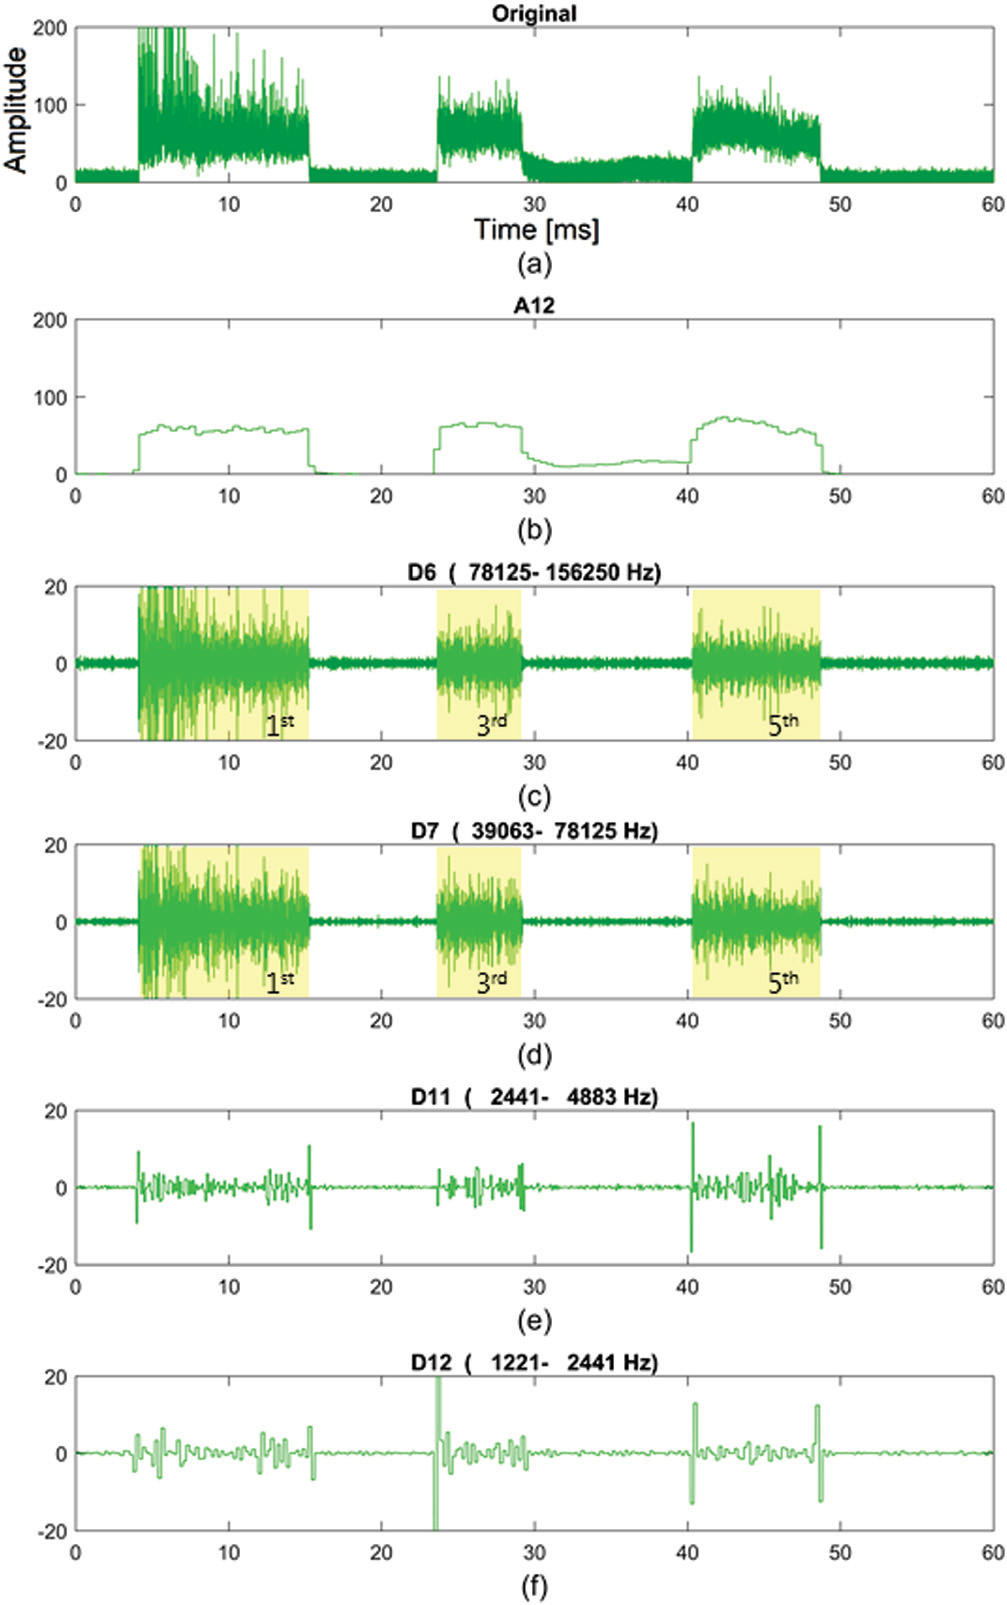
\includegraphics[width=\textwidth]{figures/Wavelet2.png}
        \subcaption{Si}
    \end{minipage}
    \hfill
    \begin{minipage}[t]{0.32\textwidth}
        \centering
        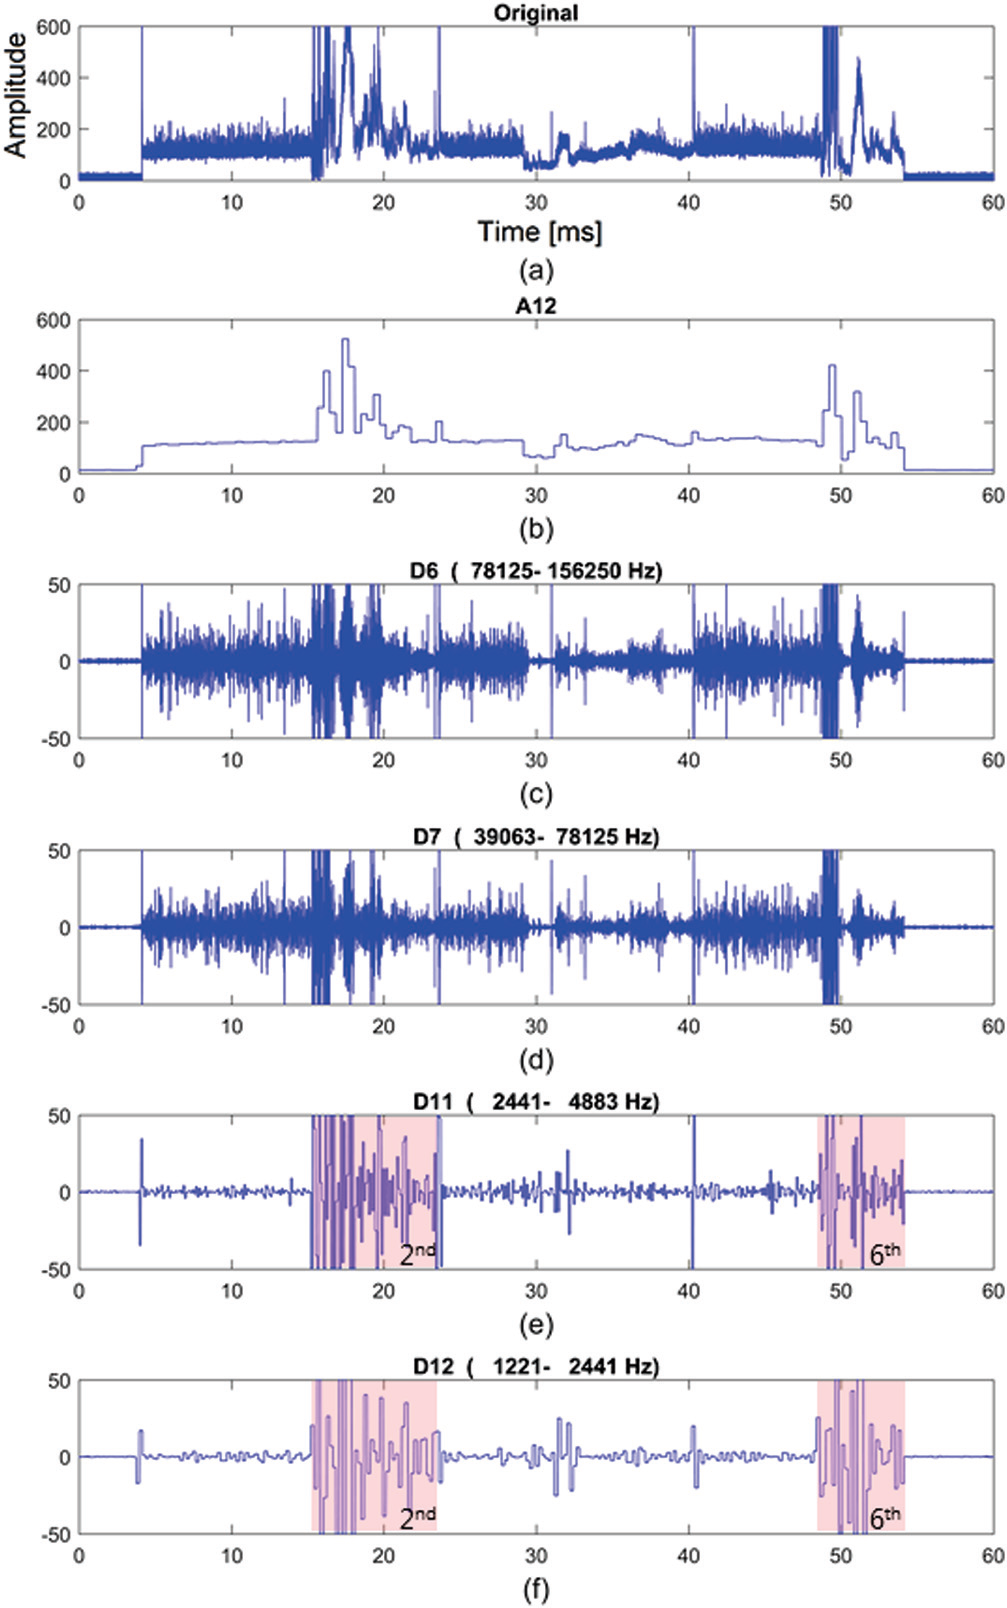
\includegraphics[width=\textwidth]{figures/Wavelet3.png}
        \subcaption{Ge}
    \end{minipage}

    \caption{Примеры результатов вейвлет-разложения оптических сигналов для датчиков на основе InGaAs, Si и Ge~\cite{vakili2017wavelet}.}
    \label{fig:three_wavelet}
\end{figure}

В работах~\cite{fang2004wavelet,sibillano2010plasma,vakili2017wavelet} показано, что временно-частотное представление лучше приспособлено к анализу кратковременных всплесков и переходных режимов, характерных для лазерной сварки. Особенно показателен пример статьи~\cite{6803929}, где для фотодиодных и спектрометрических сигналов использовалась схема в которой сначала из исходных сигналов извлекались временно-частотные коэффициенты, затем выполнялось уменьшение размерности и только после этого признаки подавались в модели классификации. Подобный подход демонстрирует важный методический переход: от одного ``понятного'' сигнала к многомерному признаковому описанию, более пригодному для автоматической диагностики.

Наряду с одномерными сигналами признаки извлекаются и из изображений. Для визуальных систем обычно используются площадь входа в парогазовый канал, длина и ширина ванны расплава, положение плазменного факела, а также число и размеры брызг~\cite{wang2020monitoring,ZHANG2019671,wu2020visual}. В этом случае извлечение признаков фактически переводит изображение в параметрическое описание, которое может быть объединено с сигналами других датчиков.

В целом этап извлечения признаков играет ключевую роль. Именно здесь исходный оптический сигнал превращается в математическое описание процесса, удобное для дальнейшей интерпретации или классификации. С одной стороны, это повышает устойчивость анализа. С другой стороны, именно на этом этапе появляется риск потери физического смысла отдельных параметров.

\subsection{Машинное обучение}

После формирования признакового пространства возникает задача автоматически связать признаки с качеством сварки, глубиной проплавления или типом дефекта. Для этого в литературе широко используются методы машинного обучения.

\subsubsection{Классические методы}

К классическим подходам относятся fuzzy logic, k-NN, SVM, FNN и BPNN. Их общая черта состоит в том, что они работают по заранее построенным признакам. Следовательно, качество результата определяется одновременно и правильностью выбора признаков, и способностью самой модели разделять состояния процесса.

Ранние примеры представлены в работах~\cite{park2001fuzzy,jauregui2008design}, где фотодиодные сигналы интерпретировались с помощью нечетких правил. Такие модели хорошо подходят для сравнительно простых задач и обладают приемлемой интерпретируемостью. Однако при росте числа признаков и дефектных состояний на первый план выходят статистические методы.

В работе~\cite{6803929} использовались FNN и SVM для оценки состояния процесса и диагностики дефектов. В статье~\cite{LEE2020307} статистические признаки спектральных сигналов классифицировались методами k-NN и SVM. В обоих случаях показано, что даже сравнительно простые алгоритмы способны обеспечить высокое качество классификации при условии удачного выбора признаков. Это важный практический вывод: для многих задач мониторинга сложность модели не обязана быть максимальной, если хорошо организован предыдущий этап обработки сигнала.

\subsubsection{Глубокое обучение}

По мере усложнения сигналов и роста числа сенсорных каналов всё большее значение приобретает глубокое обучение. Его основное преимущество состоит в способности автоматически формировать внутреннее представление данных и тем самым частично уменьшать зависимость от ручного выбора признаков.

Схематично принцип такого подхода можно записать в виде
$$
\mathbf{h} = \sigma(\mathbf{W}\mathbf{x} + \mathbf{b}),
$$
где $\mathbf{x}$ --- исходный сигнал или набор признаков, а $\mathbf{h}$ --- его скрытое представление. В работе~\cite{8756200} SAE использовался для обработки спектрометрического сигнала и показал более высокую точность, чем SVM и обычная BP-сеть. В статье~\cite{zhang2019low} похожий подход был применён уже к системе из двух фотодиодов, что особенно важно с прикладной точки зрения.

Развитие этой линии прослеживается и в многосенсорных системах. В работе~\cite{ZHANG2019671} признаки из фотодиодов, спектрометра и камер объединялись и анализировались с помощью DBN. В статье~\cite{zhang2019welding} многоканальные оптические данные использовались для распознавания дефектов на основе глубокой модели, а в~\cite{cao2023cross} для объединения различных сенсорных каналов применялся механизм cross-attention. Всё это показывает, что современные системы мониторинга всё чаще опираются не на один ``лучший'' сигнал, а на совместную обработку нескольких сигналов.

\begin{figure}[h]
    \centering
    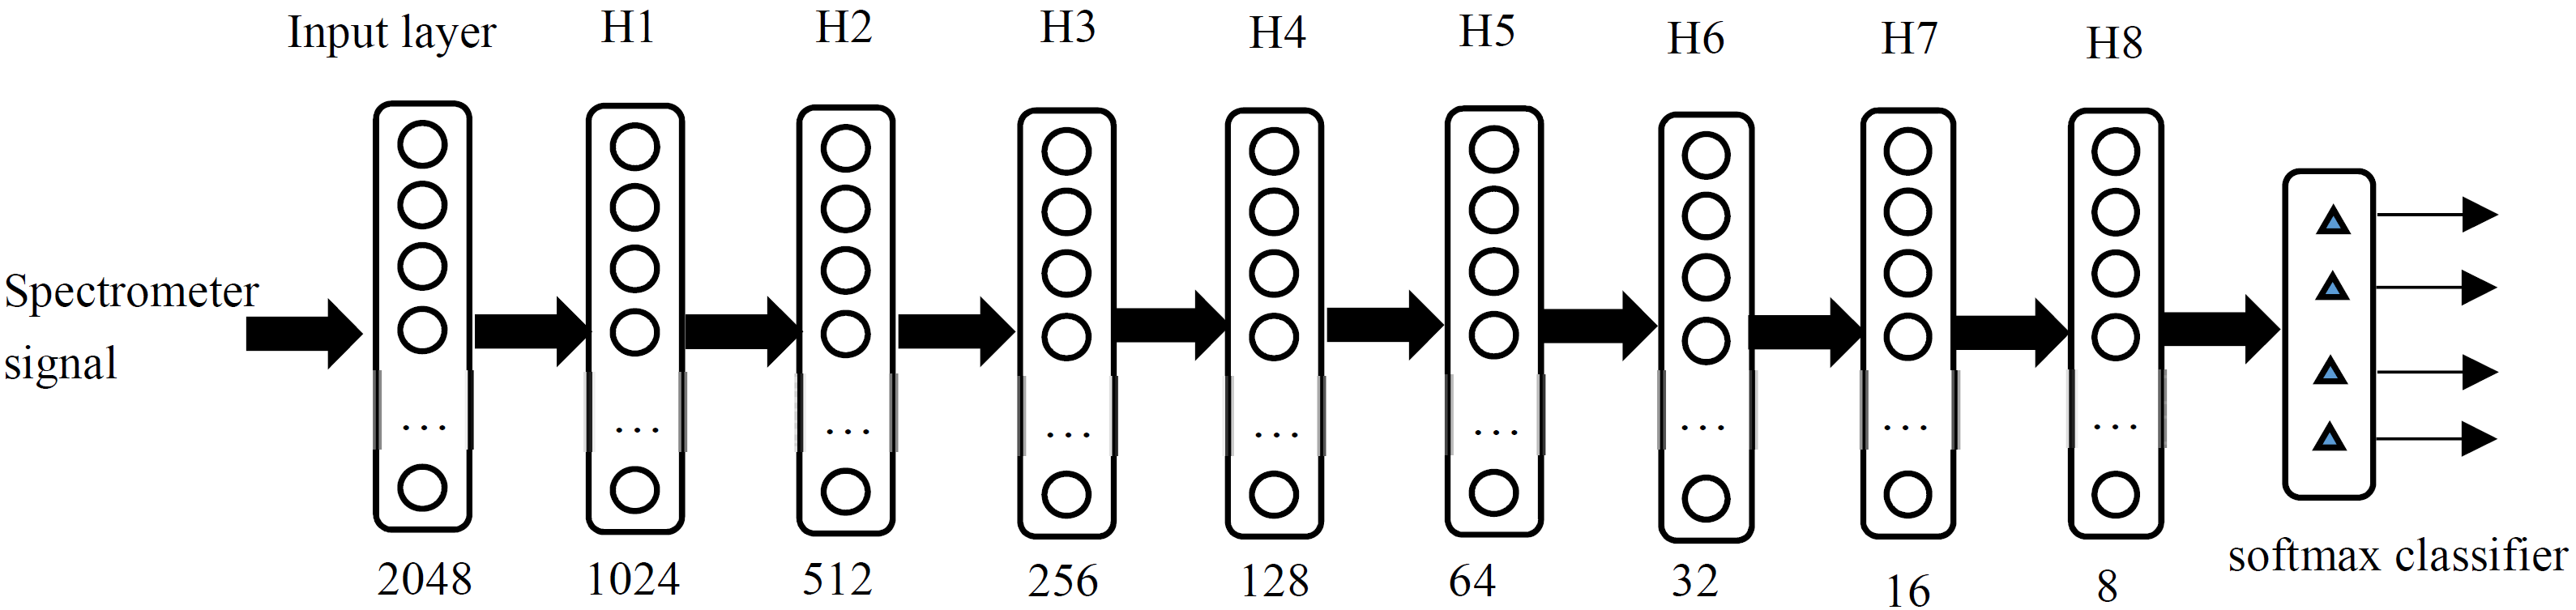
\includegraphics[width=1\textwidth]{figures/SAE.png}
    \caption{Схема архитектуры многослойного автоэнкодера (SAE)~\cite{8756200}.}
    \label{fig:neural_network_placeholder}
\end{figure}

При этом машинное обучение имеет и ограничения. Классические методы чувствительны к качеству ручного выбора признаков, а глубокие модели требуют большего объёма размеченных данных и хуже интерпретируются. Поэтому в современных обзорах подчёркивается, что наиболее надёжные решения обычно строятся на сочетании физически содержательных признаков и моделей машинного обучения~\cite{wu2022progress,huang2025laser,kouraytem2021modeling,CAI2022695}.

\subsection{Итоги рассмотрения методов анализа}

Таким образом, методы анализа оптических данных при лазерной сварке развиваются от простых и физически интерпретируемых зависимостей к многомерным признаковым описаниям и далее к моделям машинного обучения. Прямая физическая корреляция обеспечивает наибольшую прозрачность, но ограничена в универсальности~\cite{bruncko2003monitoring,sebestova2012non,konuk2011closed,mrvna2013correlation}. Извлечение признаков позволяет компактно описывать нестационарные сигналы, особенно при использовании временно-частотных методов~\cite{fang2004wavelet,vakili2017wavelet,6803929,sibillano2010plasma}. Машинное обучение, в свою очередь, обеспечивает автоматическую классификацию состояний и дефектов, а глубокие модели постепенно берут на себя и задачу формирования внутреннего представления данных~\cite{8756200,zhang2019low,ZHANG2019671,cao2023cross,zhang2019welding}.

Для настоящей работы особенно важно, что сигналы лазерной сварки следует рассматривать как нестационарные. Следовательно, их анализ не должен ограничиваться только усреднением. Кроме того, наиболее перспективным представляется сочетание сравнительно простых оптических датчиков с содержательным извлечением признаков и умеренно сложными алгоритмами анализа, сохраняющими баланс между интерпретируемостью и эффективностью.

\subsection{Заключение по обзору литературы}

Обзор литературы показывает, что качество лазерной сварки определяется сложной совокупностью взаимосвязанных явлений в зоне расплава, плазменного факела и области парогазового канала~\cite{wu2022progress,huang2025laser,konuk2011closed}. Рассмотренные работы подтверждают, что наиболее информативными для задачи мониторинга лазерной сварки являются оптические сигналы, поскольку они позволяют регистрировать как энергетическое состояние процесса, так и его геометрические и динамические проявления.

Анализ публикаций также показывает, что для мониторинга применяются разные типы оптических датчиков, прежде всего фотодиоды, спектрометры и камерные системы, причём каждый из них описывает процесс по-своему~\cite{wu2022progress,huang2025laser,zhang2019low,you2014review}. При этом решающую роль играет не только выбор датчика, но и способ обработки данных. В литературе прослеживается переход от простых физически интерпретируемых зависимостей к выделению признаков во временной, частотной и временно-частотной областях, а затем к использованию методов машинного обучения для распознавания режимов и дефектов~\cite{mrvna2013correlation,park2001fuzzy,olsson2011advances,cao2023cross}.

Таким образом, наиболее перспективным представляется подход, при котором относительно простые средства регистрации сочетаются с содержательной обработкой сигналов. Именно такая постановка позволяет использовать оптические данные не только для наблюдения за процессом, но и для оценки качества сварки в реальном времени, что и определяет направление дальнейшего исследования в настоящей работе~\cite{wu2022progress,huang2025laser}.


\endinput